\section{Methods}

\red{ What we are doing in this paper}
The Wendling model is capable of mimicking normal and seizure activity observed in hippocampal EEG in people with epilepsy~\citep{wendling2002epileptic,wendling2005interictal}. Here, the estimation of physiologically relevant model parameters from the Wendling model is considered. An unscented Kalman filter (UKF) is used to estimate the model parameters of interest. For this study, the estimation procedure is tested using EEG simulated from the Wendling model to determine the robustness of the UKF.

\subsection{Model Description and Simulation} %%%%%%%%%%%%%%%%%%%%%%%%%%%%%%%%%%%%%%%%%%%%%%%%%%%%%%%%%%%%%%%%%%%%%%%%%%%%%%%%%%%%%%%%%%%%%%%%%%%%%%%%%%%%%%%%%%%%%%%%%%%%%%%%%%%%%%%%%%%%%%%%%%%%%%%%%%%%%%%%%%%%%%%%%%%%%%%%%%%%%%%%%%%%%%%%%%%%%%%%

\red{Wendling model description.}%%%%%%%%%%%%%%%%%%%%%%%%%%%%%
The Wendling model describes the aggregate membrane potentials and firing rates produced by different neural populations. Each neural population is either excited or inhibited by other populations in the model. The net effect of one population on another is determined by a scaling constant termed connectivity. A graphical representation of the model is shown in Figure~\ref{fig: Biological}. In the model, four different neural populations are considered. The pyramidal neural population is the generator of EEG. Excitatory interneurons excite the pyramidal neurons (this connection is often modelled as a time delayed recurrent connection of the pyramidal population). Slow and fast inhibitory interneurons suppress the pyramidal neural population. The pyramidal neural population excites the excitatory and slow and fast inhibitory populations. Slow inhibitory interneurons suppress the fast inhibitory neural population. The effect of each neural population on the other is scaled by connectivity that accounts for the number of afferent synaptic connections between neural populations. A stochastic input to the model is added to account for the unknown effect of afferent pyramidal neurons from other areas of the brain.%%%%%%%%%%%%%%%%%%%%%%%%%
\begin{figure}  %%%%%%%%%%%%%%%%%%%%%%%%%%%%%%%%%%%%%%%
	\centering
		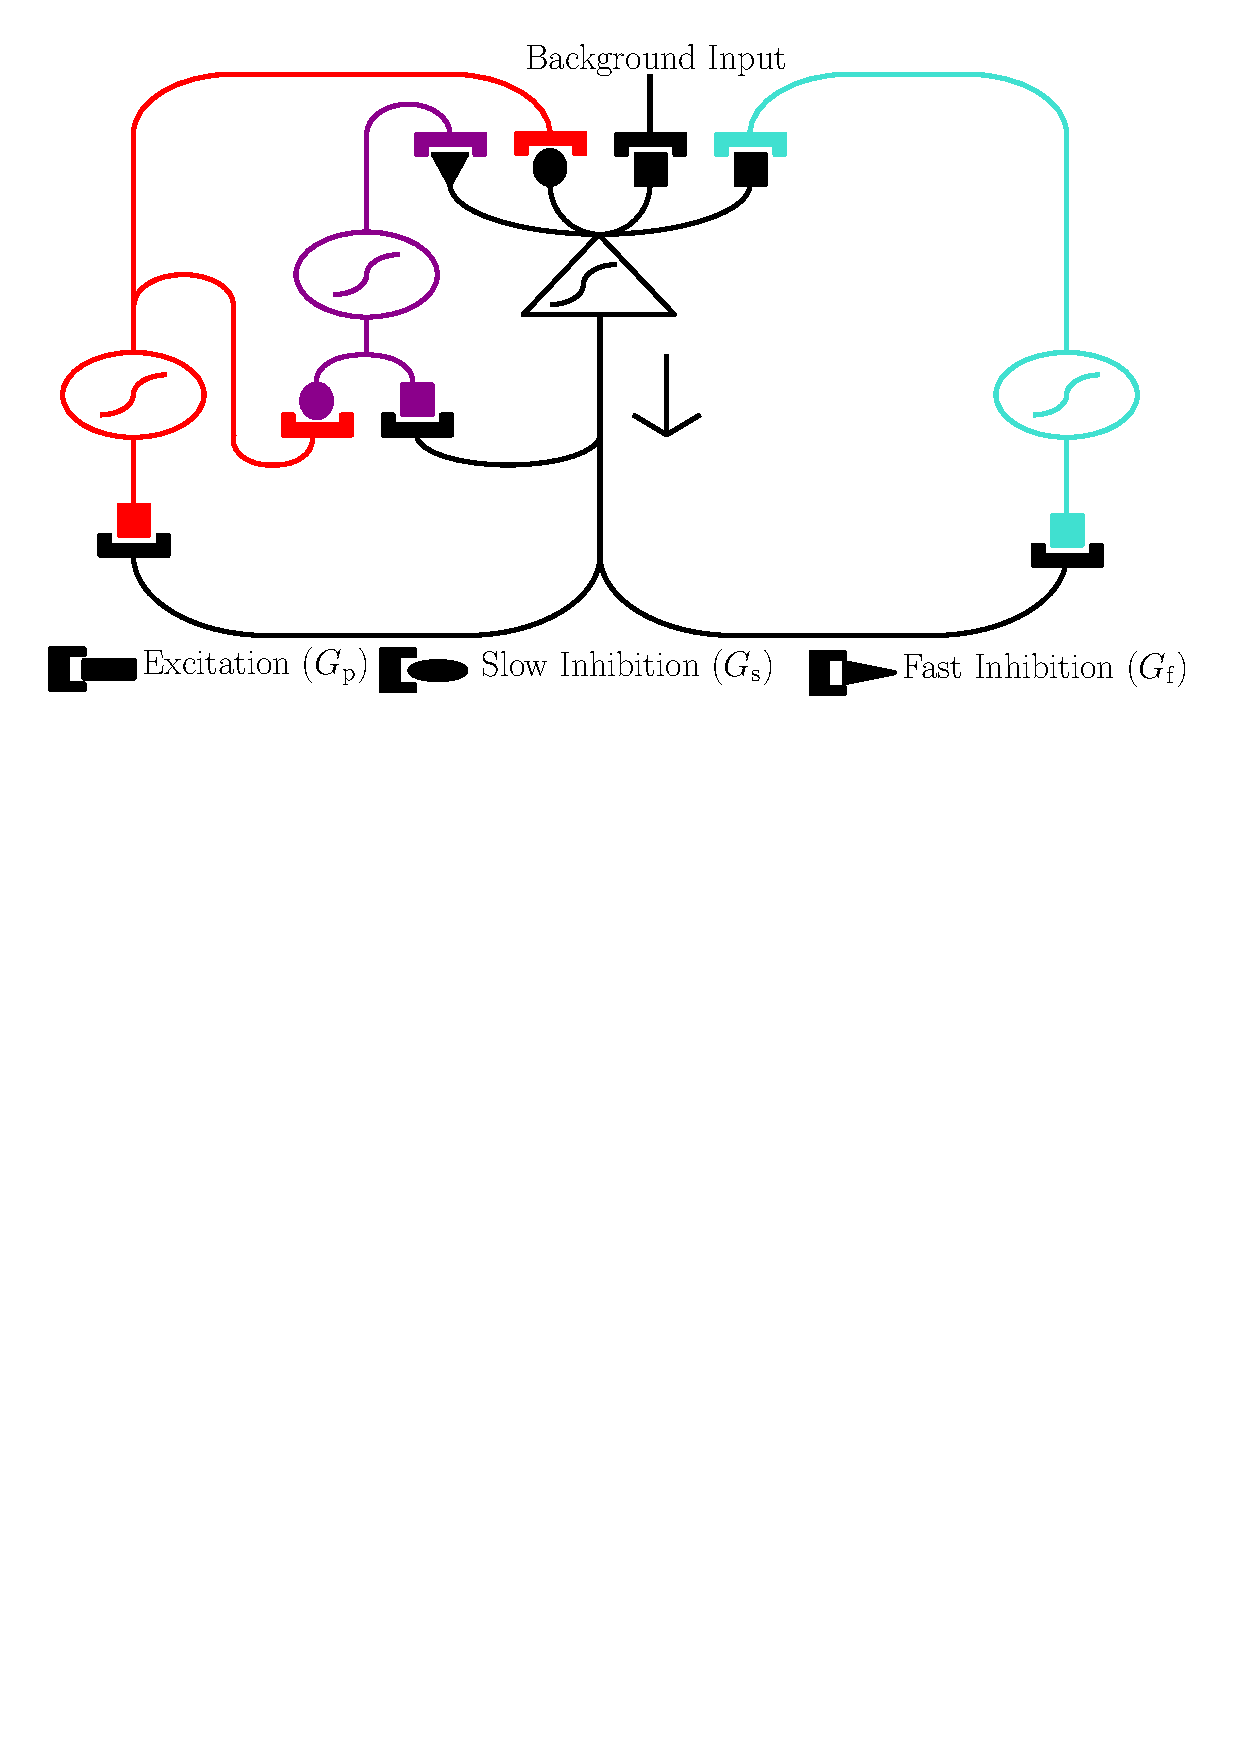
\includegraphics[width = 0.8\textwidth]{Biological1.pdf}
	\caption{Graphical Description of the Wendling model. Membrane potentials are shown and named $v_{b}$ where $b$ is p, e, f and s for pyramidal, excitatory, and fast and slow inhibitory populations, respectively. The synaptic gains of each population are specified by $G_{m}$ where $m$ is defined in the same manner as the membrane potentials and $G_{p}=G_{e}$.The triangle shape indicates the pyramidal population and the circle shapes represent interneurons. Each line indicates a neural connection, which is specified by a connectivity constant.}
	\label{fig: Biological}
\end{figure}%%%%%%%%%%%%%%%%%%%%%%%%%%%%%%%%%%%%%%%%%%%%%

\red{Mathematical functions used in the model} %%%%%%%%%%%%%%%%%%%%%%%%%%%%%%%%%%%%%%%%%%%%%%%%%%%%%%%%%%%%%%%%%%%%%%%%%%%%%%%%%%%%%%%%%%%%%%%%%%%%%%%%%%%%%%%%%%%%%%%%%%%%%%%%%%%%%%%%%%%%%%%
The Wendling model consists of two functions. The first function is a sigmoid function, which converts an aggregate membrane potential to an average firing rate,\begin{align}%%%%%%%%%%%%%%%%%%%%%%%%%%%%%%%%%%%%%%%%%%%%%
\label{eqn: Sigmoid}
g(v(t)) &= \frac{g_{max}}{1+\exp(r(v(t)-v_{0}))}, \end{align} where $g_{max}$ is the maximum the firing rate, $r$ is the sigmoid gradient, and $v_{0}$ is the membrane potential at which $0.5g_{max}$ is attained. The sigmoid function describes the response of a neuron's soma to a given membrane potential. To understand this sigmoid shape, conceptually it can be seen as the integral of a normal distribution. When considering a neural population there are numerous neurons which can be described by different sigmoid functions. The resulting sigmoid shape is a summation of the expected number of neurons that will fire given a specific membrane potential. %%%%%%%%%%%%%%%%%%%%%%%%%
The second function is an average firing rate to population membrane potential integration kernel \begin{align} %%%%%%%%%%%%%%%%%%%%%%%%%%%%%%%%%%%%%%%%%
\label{eqn: Convert}
v_{b}(t) &= G_{b}(t)h_{b}(t)*g(v(t))\\
\label{eqn: Kernel} 
h_{b}(t) &= \begin{cases} 
\frac{1}{\tau_{b}}t\exp\left(-\frac{t}{\tau_{b}}\right) & t \geq 0\\
0 & t <0
\end{cases}. \end{align} Here, $v_{b}(t)$ is the aggregate membrane potential, $h_{b}(t)$ is a kernel that converts firing rates to membrane potentials, $G_{b}(t)$ is the synaptic gain, and $\tau_{b}$ is the time constant. The operator $*$ represents a convolution. The function $h_{b}(t)$ is a time delayed exponential decay function (Figure~\ref{fig: FR2PSP_final}). The subscript $b$ is used to indicate that each neural population is described with a different synaptic gain and time constant. The synaptic gains are time dependant as they are the parameters that are altered to simulate different EEG characteristics (figure~\ref{fig: SeizureSim}). In this description of the Wendling model, numerous model parameters are considered to be stationary: the maximum firing rate~($g_{max}$), threshold voltage~($v_{0}$), sigmoid gradient ($r$), and time constants~($\tau_{b}$). 
%The assumption that the time constants are stationary is similar to assuming that neurons can be modeled as current based and not conductance based.

To solve the convolution in Equation~(\ref{eqn: Convert}), both $g(v(t))$ and $h_{m}(t)$ are transformed into the Laplace domain \begin{align}%%%%%%%%%%%%%%%%%
\label{eqn: Laplace}
G(V(s)) &= \frac{g_{\mathrm{max}}}{1+\exp(r(V(s)-v_{0}))}\\
H_{b}(s) &= \frac{\mathrm{d}}{\mathrm{d}s}\left(-\frac{G_{b}(s)}{\tau_{b}}\left(\frac{1}{s+\frac{1}{\tau_{b}}}\right)\right)\\
H_{b}(s) &= \frac{G_{b}(s)}{\tau_{b}}\left(\frac{1}{s+\frac{1}{\tau_{b}}}\right)^2.
\end{align} It is clear here that the sigmoid function has no functional dependence on time; therefore, the output of the sigmoid will be assumed to be an input firing rate~($u_{b}(t)$) where the time dependence is caused by the time varying membrane potential. The parameters $G_b(t)$ have an unknown functional dependence on time and are, therefore, assumed to be constant for this derivation. This simplifies the convolution equation to \begin{align}%%%%%%%%%%%%%%%
G(V(s)) &= U_{b}(s)\\
H_{b}(s) &= \frac{G_{b}}{\tau_{b}}\left(\frac{1}{s+\frac{1}{\tau_{b}}}\right)^2\\
\label{eqn: LaplaceNMM}
V_{b}(s) &= \frac{G_{b}U_{b}(s)}{\tau_{b}}\left(\frac{1}{s+\frac{1}{\tau_{b}}}\right)^2.
\end{align} Using Equation~(\ref{eqn: LaplaceNMM}), the membrane potential $v_{b}(t)$ can be described as a second order differential equation as follows \begin{align}%%%%%%%%%%%%%%%%%%%%%%%%%%
V_{b}(s) &= \frac{G_{b}U_{b}(s)}{\tau_{b}}\left(\frac{1}{s^2+\frac{2s}{\tau_{b}}+\frac{1}{\tau^2_{b}}}\right)\\
\label{eqn: LaplaceDiff}
V_{b}(s)\left(s^2+\frac{2s}{\tau_{b}}+\frac{1}{\tau^2_{b}}\right) &= \frac{G_{b}(s)U_{b}(s)}{\tau_{b}}.
\end{align} Taking the inverse Laplace transform of Equation~(\ref{eqn: LaplaceDiff}) results in \begin{align} %%%%%%%%%%%%%%%%%%%%%%%%%%%%%%%%
\frac{\mathrm{d}}{\mathrm{d}t^2}v_{b}(t) + \frac{\mathrm{d}}{\mathrm{d}t}\left(\frac{2*v_{b}(t)}{\tau_{b}}\right) + \frac{v_{b}(t)}{\tau^2_{b}} &= \frac{G_{b}(t)u_{b}(t)}{\tau_{b}}\\
\label{eqn: DiffNMM}
\frac{\mathrm{d}}{\mathrm{d}t^2}v_{b}(t) &= \frac{G_{b}(t)u_{b}(t)}{\tau_{b}} - \frac{\mathrm{d}}{\mathrm{d}t}\left(\frac{2*v_{b}(t)}{\tau^2_{b}}\right) -\frac{v_{b}(t)}{\tau^2_{b}}. \end{align} A dummy  variable, $z(t)$, is defined such that Equation~(\ref{eqn: DiffNMM}) can be described as two differential equations, \begin{align} %%%%%%%%%%%%%%%%%%%%%%%%%%%
\label{eqn: dummy1}
\frac{\mathrm{d}}{\mathrm{d}t}v_{b}(t) &= \dot{v}_{b}(t)\\
\label{eqn: dummy2}
\frac{\mathrm{d}}{\mathrm{d}t^2}v_{b}(t) &= \dot{z}_{b}(t)\\
\label{eqn: FR2PSP1}
\dot{v}_{b}(t)&= z_{b}(t)\\
\label{eqn: FR2PSP2}
\dot{z}_{b}(t)&=\frac{G_{b}(t)}{\tau_{b}}n_{b}u_{b}(t)-2\frac{z_{b}(t)}{\tau_{b}}-\frac{v_{b}(t)}{\tau_{b}^{2}}.
\end{align} Here $v_{b}(t)$ is the average membrane potential and $z_{b}(t)$ is its derivative. $G_{b}(t)$ and $\tau_{b}$ are the specific neural populations synaptic gain and time constant. Lastly, $u_{b}(t)$ is the firing rate to the specific neural population considered and $n_{b}$ is a constant used to describe connectivity. The term $n_{b}$ is a consequence of the model simplification, and its derivation is demonstrated in appendix~\ref{sec: AppendixA}.

\begin{figure}%%%%%%%%%%%%%%%%%%%%%%%%%%%%%%%%%%%%%%%%%%%%%%%%%
	\centering
		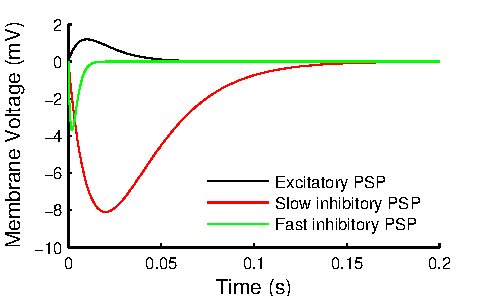
\includegraphics{FR2PSP.pdf}
	\caption{Impulse response of the firing rate to aggregate membrane potential function. The time constants and synaptic gains used for this figure correspond to that of background EEG~\citep{wendling2002epileptic}. The peaks of each response occur at time $\tau_{b}$ and the maximum membrane potential is $\exp(-1)G_{b}$, where $b$ is replaced by p, s and f for excitatory, and slow and fast inhibitory time constants and gains, respectively. The inhibitory populations response is shown as negative, as this is its net effect on the system.}
	\label{fig: FR2PSP_final}
\end{figure} %
\begin{figure}
\centering
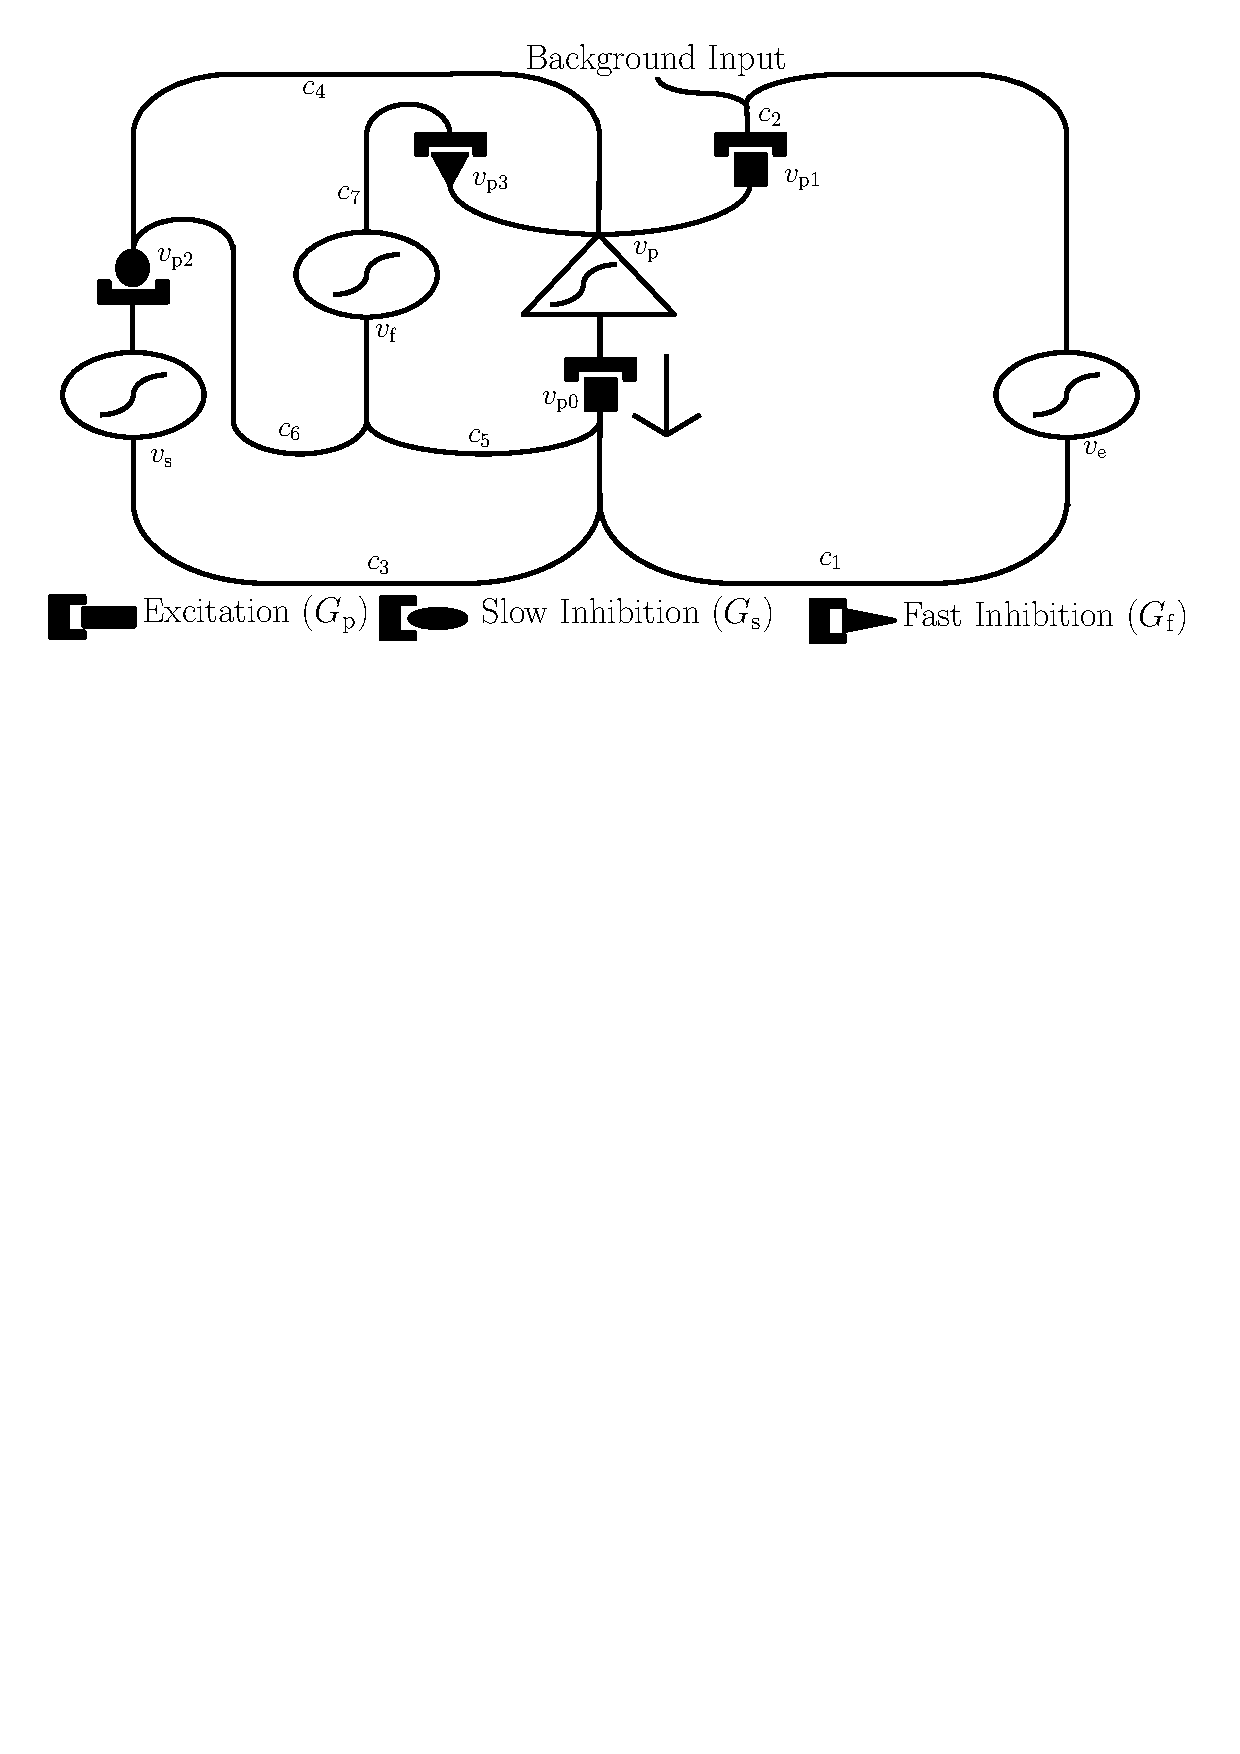
\includegraphics[width = 0.8\textwidth]{BiologicalSimplified.pdf}
\caption{Simplified graphical description of the Wendling model.}
\label{fig: BiologicalSimplified}
\end{figure}

\red{Full mathematical description of the model}
Using Equations~(\ref{eqn: FR2PSP1})-(\ref{eqn: FR2PSP2}) and observing that each synapse of the model (totaling 8), shown in figure~\ref{fig: Biological} requires two differential equations, the number of equations expected would be sixteen. However, this model can be simplified, see Appendix~\ref{sec: AppendixA},~(Figure~\ref{fig: BiologicalSimplified}) to a set of eight stochastic differential equations: \begin{align}%%%%%%%%%%%%%%%%%%%%%%%%%%%%%%%%%%%%%%%
\mathrm{d}v_{\mathrm{p0}}(t)&= z_{\mathrm{p0}}(t)\mathrm{d}t\\
\mathrm{d}z_{\mathrm{p0}}(t)&=\left(\frac{G_{\mathrm{p}}(t)}{\tau_{\mathrm{p}}}n_{\mathrm{p}}g(v_{\mathrm{p}}(t))-2\frac{z_{\mathrm{p0}}(t)}{\tau_{\mathrm{p}}}-\frac{v_{\mathrm{p0}}(t)}{\tau_{\mathrm{p}}^{2}}\right)\mathrm{d}t\\
\mathrm{d}v_{\mathrm{p1}}(t)&= z_{\mathrm{p1}}(t)\mathrm{d}t\\
\label{eqn: Wiener}
\mathrm{d}z_{\mathrm{p1}}(t)&=\left(\frac{G_{\mathrm{e}}(t)}{\tau_{\mathrm{e}}}(\mu +n_{\mathrm{e}}g(v_{\mathrm{e}}(t))-2\frac{z_{\mathrm{p1}}(t)}{\tau_{\mathrm{e}}}-\frac{v_{\mathrm{p1}}(t)}{\tau_{\mathrm{e}}^{2}}\right)\mathrm{d}t + \frac{G_{\mathrm{e}}(t)}{\tau_{\mathrm{e}}}\epsilon(t)\mathrm{d}W\\
\mathrm{d}v_{\mathrm{p2}}(t)&= z_{\mathrm{p2}}(t)\mathrm{d}t\\
\mathrm{d}z_{\mathrm{p2}}(t)&=\left(\frac{G_{\mathrm{s}}(t)}{\tau_{\mathrm{s}}}n_{\mathrm{s}}g(v_{\mathrm{s}}(t))-2\frac{z_{\mathrm{p2}}(t)}{\tau_{\mathrm{s}}}-\frac{v_{\mathrm{p2}}(t)}{\tau_{\mathrm{s}}^{2}}\right)\mathrm{d}t\\
\mathrm{d}v_{\mathrm{p3}}(t)&= z_{\mathrm{p3}}(t)\mathrm{d}t\\
\mathrm{d}z_{\mathrm{p3}}(t)&=\left(\frac{G_{\mathrm{f}}(t)}{\tau_{\mathrm{f}}}n_{\mathrm{f}}g(v_{\mathrm{f}}(t))-2\frac{z_{\mathrm{p3}}(t)}{\tau_{\mathrm{f}}}-\frac{v_{\mathrm{p3}}(t)}{\tau_{\mathrm{f}}^{2}}\right)\mathrm{d}t.
\end{align} In these equations $dW$ represents a Wiener process \iref and is required as $\epsilon(t)\sim N(0,\sigma)$, where $\sigma$ and $\mu$~(Eq.~(\ref{eqn: Wiener})) describe the mean and variance of the stochastic model input, respectively. Further, $v_{\mathrm{p0-3}}(t)$ represent the membrane potential produced by a specific populations synapse and $z_{\mathrm{p0-3}}(t)$ their derivatives. The inputs to each neural population are specified by $v_{b}(t) $, and are the membrane potential of the specific population, where $b$ takes the values of p, e, s and f representing pyramidal, excitatory, and slow and fast inhibitory populations, respectively. Therefore $v_{\mathrm{p}}(t) $ is the output of the model. All $v_{b}(t) $ can be described in terms of $v_{\mathrm{p0-3}}(t)$ as follows \begin{align}%%%%%%%%%%%%%%%%%%%%%%%%%%%%%%%%%%%%%%%%%%%%%%%%%%%%%%%%%%%%%%%%
v_{\mathrm{p}}(t) &= v_{\mathrm{p1}}(t)-c_{4}v_{\mathrm{p2}}(t)-v_{\mathrm{p3}}(t)\\
v_{\mathrm{e}}(t) &= c_{1}v_{\mathrm{p0}}(t)\\
v_{\mathrm{s}}(t) &= c_{3}v_{\mathrm{p0}}(t)\\
v_{\mathrm{f}}(t) &= c_{5}v_{\mathrm{p0}}(t)-c_{6}v_{\mathrm{p2}}(t),
\end{align} where $c_{1}$, $c_{3}$ and $c_{5}$ represent the connectivity strength from pyramidal to excitatory, slow inhibitory and fast inhibitory populations, respectively. The last two connectivity terms, $c_{4}$ and $c_{6}$, represent the connectivity strength from the slow inhibitory to the excitatory and fast inhibitory populations, respectively. Finally, all $n_{b}$ can be defined as connectivity constants:\begin{align}%%%%%%%%%%%%%%%%%%%%%%%%%%%%%%%%%%%%%%%%%%%
n_{p} &=1\\
n_{\mathrm{e}} &=c_{2}\\
n_{\mathrm{s}} &=1\\
n_{\mathrm{f}} &=c_{7},
\end{align} where $c_{2}$ and $c_7$ represent the connectivity strength from excitatory and fast inhibitory populations to the pyramidal population.
\begin{figure}%%%%%%%%%%%%%%%%%%%%%%%%%%%%%%%%%%%%%%%%%%%%%%%%%%%%%%%%%%%%%
	\centering
	    \begin{tabular}{p{0.05cm} l}
    \imagetop{(A)} & \imagetop{\includegraphics[width=0.8\textwidth]{InsetF1.pdf}} \\
    \imagetop{(B)} & \imagetop{\includegraphics[width=0.8\textwidth]{Single_iEEG_Trace_TTN.pdf}}
    \end{tabular}
%\subfigure[]	{\includegraphics{pdf/InsetF1.pdf}
%}\\
%\subfigure[]{	\includegraphics[width =1\textwidth]{pdf/Single_iEEG_Trace_TTN.pdf}
%}\\
	\caption{Simulated seizure using the Wendling model compared to a seizure recorded from an \textsl{in vivo} model of epilepsy.. (a) Here four different sets of synaptic gains are used to simulate the seizure. Four types of neural activity are demonstrated in this figure: background EEG (1-10s), interictal (11-20s), low voltage high frequency (21-30s) and seizure (31-40s). The last ten seconds shows background data again. Four insets are demonstrated in the figure each corresponding to a different type of activity. The insets in order from left to right show: background, interictal, low voltage high frequency and seizure activity. (b) Tetanus toxin focal seizure data, where four types of activity are demonstrated: background(1-5s), interictal (6-20s), low voltage high frequency (21-35s) and seizure (36-60s).}
	\label{fig: SeizureSim}
\end{figure}%%%%%%%%%%%%%%%%%%%%%%%%%%%%%%%%%%%%%%%%%%%%%%%%%%%%%%%%%%%%%%%%%%%%%%


\red{Simulation of model}
This set of continuous stochastic differential equations is discretised using Euler-Mariyama's method \iref, to simulate EEG \begin{align}
\label{eqn: EulerW1}
v_{\mathrm{p0},k+1}&=v_{\mathrm{p0},k}+Tz_{\mathrm{p0},k}\\
z_{\mathrm{p0},k+1}&=z_{\mathrm{p0},k}+T\left(\frac{G_{p,k}}{\tau_{p}}n_{p}g(v_{p,k})-2\frac{z_{\mathrm{p0},k}}{\tau_{p}}-\frac{v_{\mathrm{p0},k}}{\tau_{p}^{2}}\right)\\
v_{\mathrm{p1},k+1}&=v_{\mathrm{p1},k}+Tz_{\mathrm{p1},k}\\
z_{\mathrm{p1},k+1}&=z_{\mathrm{p1},k}+T\left(\frac{G_{\mathrm{e},k}}{\tau_{\mathrm{e}}}(\mu +n_{\mathrm{e}}g(v_{\mathrm{e},k})-2\frac{z_{\mathrm{p1},k}}{\tau_{\mathrm{e}}}-\frac{v_{\mathrm{p1},k}}{\tau_{\mathrm{e}}^{2}}\right) + \sqrt{t}\frac{G_{\mathrm{e},k}}{\tau_{\mathrm{e}}}\epsilon_{t}\\
v_{\mathrm{p2},k+1}&=v_{\mathrm{p2},k}+Tz_{\mathrm{p2},k}\\
z_{\mathrm{p2},k+1}&=z_{\mathrm{p2},k}+T\left(\frac{G_{\mathrm{s},k}}{\tau_{\mathrm{s}}}n_{\mathrm{s}}g(v_{\mathrm{s},k})-2\frac{z_{\mathrm{p2},k}}{\tau_{\mathrm{s}}}-\frac{v_{\mathrm{p2},k}}{\tau_{\mathrm{s}}^{2}}\right)\\
v_{\mathrm{p3},k+1}&=v_{\mathrm{p3},k}+Tz_{\mathrm{p3},k}\\
\label{eqn: EulerW8}
z_{\mathrm{p3},k+1}&=z_{\mathrm{p3},k}+T\left(\frac{G_{\mathrm{f},k}}{\tau_{\mathrm{f}}}n_{\mathrm{f}}g(v_{\mathrm{f},k})-2\frac{z_{\mathrm{p3},k}}{\tau_{\mathrm{f}}}-\frac{v_{\mathrm{p3},k}}{\tau_{\mathrm{f}}^{2}}\right),
\end{align} where $k$ represents the current sample and $T$ is the period between them. The static parameter values are shown in Table~\ref{tab: Static}. The variance of the input,$\sigma$, is specified such that 99.7\% of realisations drawn from the Gaussian distribution fall within the specified maximum and minimum firing rate. For the cases where the realisations from the Gaussian distribution are not contained within the limits specified, the specific sample of interest is redrawn from the same Gaussian distribution until the firing rate falls within the specified range. In Table~\ref{tab: Static}, the parameters $G_{\mathrm{p},k}$, $G_{\mathrm{e},k}$, $G_{\mathrm{s},k}$ and $G_{\mathrm{f},k}$ are not specified as these parameters will vary for different simulations. However, for this simulation, it is assumed that \begin{align}
G_{\mathrm{p},k} = G_{\mathrm{e},k}.
\end{align} This assumption can be made as the excitatory population in this model specifies recurrent connections between pyramidal neurons.  
\singlespacing
\small
\begin{center}%%%%%%%%%%%%%%%%%%%%%%%%%%%%%%%%%%%%%%%%%%
	\begin{table}
			\caption{Static Model Parameters~\citep{wendling2002epileptic}. Here p, e, s and f represent populations of pyramidal neurons and excitatory, and slow and fast inhibitory interneurons, respectively.}
		\begin{tabular}{||p{4cm}|p{6cm}|p{1.5cm}|p{1.2cm}||}\hline
			 \textsc{Model parameter}  & \textsc{Physical description} & \textsc{Value} & \textsc{Units}  \\\hline\hline
			 $\tau_{p}$ & Time constant for pyramidal neurons & 100 & $s^{-1}$\\\hline
			 $\tau_{\mathrm{e}}$ & Time constant for excitatory neurons & 100 & $s^{-1}$\\\hline
			 $\tau_{\mathrm{s}}$ & Time constant for slow inhibitory neurons & 35 & $s^{-1}$\\\hline
			 $\tau_{\mathrm{f}}$ & Time constant for fast inhibitory neurons & 500 & $s^{-1}$\\\hline
			 $c$ & Connectivity constant & 135 & NA\\\hline
			 $c_{1}$ & Connectivity constant (p - e) & $c$ & NA \\\hline
			 $c_{2}$ & Connectivity constant (e - p) & $0.8c$ & NA\\\hline
			 $c_{3}$ & Connectivity constant (p - s) & $0.25c$ & NA \\\hline
			 $c_{4}$ & Connectivity constant (s - p)& $0.25c$ & NA\\\hline
			 $c_{5}$ & Connectivity constant (p - f) & $0.3c$ & NA\\\hline
			 $c_{6}$ & Connectivity constant (s - f) & $0.1c$ & NA\\\hline
			 $c_{7}$ & Connectivity constant (f - p) & $0.8c$ & NA\\\hline
			 $g_{max}$ & Maximum firing rate & 5 & Hz \\\hline
			 $v_{0}$ & PSP for which 50\% firing rate is achieved & 6 & $mV^{-1}$\\\hline
			 $r$ & Gradient of sigmoid function & 0.56 & NA \\\hline
			 $f_{max}$ & Maximum input firing rate & 150 & Hz \\\hline
			 $f_{min}$ & Minimum input firing rate & 30 & Hz \\\hline
			 $\mu$ & Input mean firing rate & 90 & $Hz$\\\hline
			 $\sigma$ & Variance of input firing rate & 15 & $Hz$\\\hline\hline 
		\end{tabular}
		\label{tab: Static}
	\end{table}
\end{center}%%%%%%%%%%%%%%%%%%%%%%%%%%%%%%%%%%%%%%%%%%%%%%%%%%%%%%%%%%
\onehalfspacing

\subsection{Estimation}

\red{Generic description on a nonlinear system}
A generic system is defined where \begin{align}
\label{eqn: NonlinEstS}
\mathbf{\dot{x}}(t) &= \mathbf{A}(\mathbf{x}(t),\mathbf{\theta}(t)) + \mathbf{B}(\mathbf{u}(t)) + \mathbf{n}(t)\\
\label{eqn: NonlinEstO}
\mathbf{y}(t)  &= \mathbf{C}(\mathbf{x}(t)) +\mathbf{D}(\mathbf{u}(t))+\mathbf{r}(t),
\end{align} where boldface indicates a matrix or vector. Here, $\mathbf{x}(t)$ is the state vector and $\dot{\mathbf{x}}(t)$ is its derivative, where
\[ \mathbf{\dot{x}}(t) = \left[ \begin{array}[pos]{c}
\dot{x}_{1}(t)\\
\vdots \\
\dot{x}_{n}(t) \end{array} \right] .\] $\mathbf{A}$ and $\mathbf{B}$ are the state and input functions, respectively and $\mathbf{u}(t)$ is the input to the model. $\mathbf{C}$ and $\mathbf{D}$ are the output and input-to-output functions, respectively. The output of the model is $\mathbf{y}(t)$ with $\mathbf{n}(t)$ the model uncertainty, and $\mathbf{r}(t)$ the observation noise. Here, $\mathbf{n}(t)$ takes into account that the model is not a perfect descriptor of the modeled system as well as accounting for unknown inputs to the system, and $\mathbf{r}(t)$ describes the maximum amplitude of the noise in the observations. Both $\mathbf{n}(t)$ and $\mathbf{r}(t)$ are zero mean Gaussian distributed with a system dependant variance. The assumption of Gaussian distribution is only valid when the number of samples for the estimation procedure is large (central limit theorem \iref). In particular, the sampling rate needs to be much greater than the maximum frequency that the model dynamics describes. This is often referred to as an oversampled system \iref.

\red{Introduction to the UKF}
Estimation algorithms usually estimate the model states, $\mathbf{x}(t)$, given some observation, $\mathbf{y}(t)$ . One method that is often used for estimating linear systems is the Kalman filter. The Kalman filter consists of two steps: prediction and correction. In the prediction step, model states are propagated through the system and are used to determine the expected value of the states at the next time step. Using a first order Euler-Maruyama method, this can be described by \begin{align}
\label{eqn: StateProgL}
\mathbf{x}_{k+1}^{-} &= \mathbf{x}_{k} + T(\mathbf{A}\mathbf{x}_{k} +\mathbf{B}\mathbf{u}_{k})+\sqrt{T}\mathbf{n}_{k}\\
\label{eqn: YProp}
\mathbf{y}_{k+1}^{-}  &= \mathbf{y}_{k} + T(\mathbf{C}\mathbf{y}_{k}+\mathbf{D}\mathbf{u}_{k}) +\sqrt{T}\mathbf{r}_{k},
\end{align} where the subscript in $\mathbf{x}_{k}^{-}$ is used to indicate the current sample and $T$ is the sampling period. The stochastic variables are $\mathbf{n}_{k}\sim N(0,\mathbf{\sigma}_{n})$ and $\mathbf{r}_{k}\sim N(0,\mathbf{\sigma}_{r})$, where $\mathbf{\sigma}_{n}$ and $\mathbf{\sigma}_r$ are the standard deviations for each respective noise process and $N(\cdot)$ is a Gaussian distribution. The superscript in $\mathbf{x}_{k}^{-}$ is used to indicate that this estimate is a prediction that has not yet been corrected by the current observation. Performing this kind of prediction for a nonlinear system would be inaccurate as the propagation of states like this in a system would require the assumption that the maximum error in the states remains constant for all time. However, in a nonlinear system this is not true, as a state's error can change from one prediction to the next. In particular, if the original state estimate is incorrect in a nonlinear system it is possible that the error can increase in the next iteration of the estimation procedure. In order to account for this error, or the altering of state covariance, an unscented filter is used in the prediction step for nonlinear systems. The advantage of an unscented filter over local linearisation techniques is that speed is improved and discontinuities can be handled. 

\red{The unscented filter}
The unscented filter is completely described by a state's mean and covariance such that:\begin{align}
\label{eqn: Unscented_Transform1}
\mathbf{\mathcal{X}}_{n} &= \mathbf{\overline{x}}_{k} + (\sqrt{\kappa+D_{x}\mathbf{P_{xx,k}}})_{n} \quad n=1,\hdots,D_x\\
\label{eqn: Unscented_Transform2}
\mathbf{\mathcal{X}}_{n+D_{x}} &= \mathbf{\overline{x}}_{k} - (\sqrt{\kappa+D_{x}\mathbf{P_{xx,k}}})_{n} \quad n=1,\hdots,D_x,\\
\label{eqn: Unscented_TransformY1}
\mathbf{\mathcal{Y}}_{n} &= \mathbf{\overline{y}}_{k} + (\sqrt{\kappa+D_{y}\mathbf{P_{yy,k}}})_{n} \quad n=1,\hdots,D_y\\
\label{eqn: Unscented_TransformY2}
\mathbf{\mathcal{Y}}_{n+D_{y}} &= \mathbf{\overline{y}}_{k} - (\sqrt{\kappa+D_{y}\mathbf{P_{yy,k}}})_{n} \quad n=1,\hdots,D_y,
\end{align} where $\mathbf{\overline{x}}_{k}$ and $\mathbf{\overline{y}}_{k}$ are the current state estimate and observation. $(\sqrt{\cdot})_{n}$ denotes the $n$th row of the matrix square root. $D_{x}$ and $D_{y}$ indicate the number of states in the system and the number of observations. Covariance matrices, $\mathbf{P_{xx,k}}$ and $\mathbf{P_{yy,k}}$, are the expected error of the current state and observation. The points $\mathbf{\mathcal{X}}$ are called sigma points and represent the states one standard deviation away for the estimated mean. The term $\kappa$ is a predefined constant, which determines the relative effect of the propagation of the mean. If $\kappa$ is equal to zero then the system mean is not propagated as a sigma point. However, if $\kappa$ is greater than zero then \begin{align}
\mathbf{\mathcal{X}}_{0} &= \mathbf{\overline{x}}_{k}.
\end{align} Therefore, 2$D_{x}$ sigma points are assigned when $\kappa$ is zero and 2$D_{x}$+1 sigma points are assigned when it is greater than zero. The sigma points are propagated through the system in order to update the expectation about the state mean and error: \begin{align}%%%%%%%%%%%%%%%%%%%%%%%%%%%%%%%%%%%%
\mathbf{\mathcal{X}}_{n,k+1} &= \mathbf{\mathcal{X}}_{n,k}+ T(\mathbf{A}(\mathbf{\mathcal{X}}_{n,k}) +\mathbf{B}(\mathbf{u}_{k})) +\sqrt{T}{n}_{k}\\
\overline{\mathbf{x}}_{k+1}^{-} &= \frac{1}{2D_{x}+\kappa}\sum_{n=1}^{2D_{x}} \mathbf{\mathcal{X}}_{n,k+1}\\
\mathbf{P}_{xx,k+1}^{-} &= \frac{1}{2D_{x}+\kappa}\sum_{n=1}^{2D_{x}} (\mathbf{\mathcal{X}}_{n,k+1} -\mathbf{\overline{x}}_{k+1}^{-})(\mathbf{\mathcal{X}}_{n,k+1}-\mathbf{\overline{x}}_{k+1}^{-})^{\top} + \mathbf{Q}.%%%%%%%%%%%%%%%%%%%%%%%%%%%%%%%%%%%%
\end{align} $\overline{\mathbf{x}}_{k+1}^{-}$ and $\mathbf{P}_{xx,k+1}^{-}$ are the predictions for the state and state covariance matrices. The negative superscript is used to indicate an uncorrected prediction. The term $\mathbf{Q}$ is the expectation of the model error $n_{k}$ and $(\cdot)^{\top}$ indicates the transpose. It is now possible to make a prediction about the observation at sample $k+1$ by propagating the sigma points through Equation~(\ref{eqn: YProp}) \begin{align} %%%%%%%%%%%%%%%%%%%%%%%%%%%%
\mathbf{\mathcal{Y}}_{n,k+1} &= \mathbf{\mathcal{Y}}_{n,k} + T(\mathbf{C}(\mathbf{\mathcal{X}}_{n,k+1})+ \mathbf{D}(\mathbf{u}_{k}))+ \sqrt{T}\mathbf{r}_{k}\\
\overline{\mathbf{y}}_{k+1}^{-} &= \frac{1}{2D_{x}+\kappa}\sum_{n=1}^{2D_{x}} \mathbf{\mathcal{Y}}_{n,k+1}\\
\label{eqn: statecovg}
\mathbf{P}_{xy,k+1}^{-} &= \frac{1}{2D_{x}+\kappa}\sum_{n=1}^{2D_{x}} (\mathbf{\mathcal{X}}_{n,k+1}-\overline{\mathbf{x}}_{n,k+1}) (\mathbf{\mathcal{Y}}_{n,k+1}-\overline{\mathbf{y}}_{k+1}^{-})^{\top}\\
\mathbf{P}_{yy,k+1}^{-} &= \frac{1}{2D_{x}+\kappa}\sum_{n=1}^{2D_{x}} (\mathbf{\mathcal{Y}}_{n,k+1}-\overline{\mathbf{y}}_{k+1}^{-}) (\mathbf{\mathcal{Y}}_{n,k+1}-\overline{\mathbf{y}}_{k+1}^{-})^{\top} +\mathbf{R},%%%%%%%%%%%%%%%%%%%%%%%%%%%%%%%%%%%%%%%%%%%%
\end{align} where $\overline{\mathbf{y}}_{k+1}^{-}$ and $\mathbf{P}_{yy,k+1}^{-}$ are the predictions for the model output and its covariance, respectively. $\mathbf{P}_{xy,k+1}^{-}$ is the covariance matrix of the states and observations and $\mathbf{R}$ is the expectation of the observation error $\mathbf{r}_{k}$.

\red{How states are predicted using the unscented transform}
The predictions of the states,$\overline{\mathbf{x}}_{k+1}^{-}$, and observations, $\overline{\mathbf{y}}_{k+1}^{-}$, now need to be corrected based on the observations. This is achieved by determining the Kalman gain and updating the predictions based on the current observation: \begin{align}
\mathbf{K} &= \mathbf{P}_{xy,k+1}^{-}(\mathbf{P}_{yy,k+1}^{-})^{-1}\\
\overline{\mathbf{x}}_{k+1} &= \overline{\mathbf{x}}_{k+1}^{-} + \mathbf{K}(\mathbf{y}_{k+1}-\overline{\mathbf{y}}_{k+1}^{-})\\
\mathbf{P}_{xx,k+1} &= \mathbf{P}_{xx,k+1}^{-} - \mathbf{K}(\mathbf{P}_{xy,k+1}^{-})^{\top},
\end{align} where $\mathbf{y}_{k}$ is the observation, $\overline{\mathbf{x}}_{k+1}$ is the corrected estimate of the state and $\mathbf{P}_{xx,k+1}$ is the estimate of its error. This set of equations describes the UKF and how it can be used to estimate states. However, for this study, estimation of states and parameters is required (dual estimation).

\red{Definition of slow state matrix and its dynamics}
The parameters that are being estimated are $G_{\mathrm{p},k}$, $G_{\mathrm{e},k}$, $G_{\mathrm{s},k}$ and $G_{\mathrm{f},k}$, where it is assumed that \begin{align}
G_{\mathrm{p},k} = G_{\mathrm{e},k}.
\end{align} Therefore, three parameters need to be estimated, and a parameter matrix is defined
\[ \mathbf{\theta}_{k} = \left[ \begin{array}[pos]{c}
G_{\mathrm{p},k}\\
G_{\mathrm{s},k} \\
G_{\mathrm{f},k} \end{array} \right] .\] The original state matrix is then augmented with the parameter matrix 
\[ \mathbf{x}_{k} = \left[ \begin{array}[pos]{c}
\mathbf{x}_{k}\\
\mathbf{\theta}_{k} \end{array} \right] .\] The change in model parameters occurs at a longer time scale than the model states. Therefore, for convenience, the model states and parameters are referred to as fast and slow states. The next issue to consider is the description of the dynamics for the slow states. Due to the prediction correction steps of the unscented Kalman filter these slow states can be assigned trivial dynamics such that
\begin{align}
\label{eqn: parameterdynamics}
\mathbf{\theta}_{k+1} &= \mathbf{\theta}_{k} + \mathbf{\eta_{k}}\\
E(\mathbf{\theta}_{k+1}) &= \mathbf{\theta}_{k}\\
P_{\mathbf{\theta} \mathbf{\theta},k+1} &= \mathbf{\Psi},
\end{align} where $E(\cdot)$ is the expectation function and $\mathbf{\eta}_{k} \sim N(0,\mathbf{\sigma})$.

\red{Intialisation of UKF for stationary parameters}
When initialising the unscented Kalman filter the model uncertainty and initialisation standard deviation for each state needs to be specified. To determine the accuracy of the model when estimating fast states, initial estimations are performed under the assumption that the model's slow states are stationary. Assuming that the model slow states are stationary allows for the uncertainty in these states to remain low. This uncertainty characterises possible model inaccuracy, and also allows the slow state to slowly vary until they converges to their true values. Standard deviations in the estimation description are described such that one standard deviation from the midpoint of the specified slow states range encompasses all possible values for the particular state. Further, the uncertainty of states directly affected by the stochastic model input is increased to account for the unpredictable nature of this signal when simulating. This is required as a stochastic process cannot be estimated accurately. 

Due to the stochastic model input, it is non-trivial to determine the maximum limit of the physiological range describing the fast states. Therefore, numerous simulations are performed and the resulting mean and standard deviation for each state is used as the initial mean and standard deviation for estimation: \begin{align}
v_{b,0} = \frac{1}{n}\sum\limits_{i=1}^n E(v_{i,b,k}), \end{align} where $n$ indicates the number of simulations performed and $v_{b,0}$ and $E(v_{b,k,i})$ indicate the expected value of the initialised fast states and the expected value of each simulation, respectively. For the standard deviation, the average over multiple simulations for a normal distribution can be determined by \begin{align}
\sigma^2_{b,0} = \frac{1}{n-1}\sum\limits_{i=1}^n \sigma^2_{b,k},\end{align} where $\sigma^2_{b,0}$ and $\sigma^2_{b,k}$ are the variances of the initial guess and of each state's simulation results, respectively.


Next the assignment of the mean and covariance of the slow states is considered. For this calculation it is assumed that all possible values of the slow states are equally probable. The range of these slow states is infinite; however, there is a physiological bound on their values~\citep{wendling2002epileptic}. These bounds will be used and are defined as $\theta_{b,max}$ and $\theta_{b,min}$. The mean and covariance of the slow states are\begin{align}
\label{eqn: InitThetaMean}
\overline{\theta}_{b,0} = \frac{\theta_{b,max}+\theta_{b,min}}{2}\\
\label{eqn: InitThetaCoV}
P_{\theta\theta,0} = (\overline{\theta}_{b,0}-\theta_{b,min})^2.
\end{align}

\red{Intialisation of UKF for varying parameters}
When estimating slow states that vary within a single simulation, the uncertainty assigned to these parameters is increased. This increase in uncertainty guarantees that the estimation procedure will not converge to a specific slow state and remain there, but instead will track it as it varies. 

\red{Estimation of model input mean}
Finally, estimation of the stochastic input's mean to the neural mass is considered. Here it is assumed that the model input mean is varying slowly. By doing so the input mean can be augmented to the state matrix and assigned trivial dynamics. With the physiological bounds on the input specific by~\cite{wendling2002epileptic}, the initial mean and standard deviation of the input can be defined by equations~\ref{eqn: InitThetaMean}-\ref{eqn: InitThetaCoV}.

\red{Robustness test}
The performance of the estimation procedure is determined. Initially, only estimation of fast states is considered. This is then developed to the full estimation procedure where all model parameters and the input mean are estimated. The estimation procedure is then tested under numerous observation noise conditions, and with varying levels of error in the initialisation of states.
